\section{Application: fuzzgoat}
\label{sec:3-3}

% -T: Introduce fuzzgoat and it's details
In this section, we assess the performance of Waffle by fuzzing \textit{fuzzgoat}. Fuzzgoat is an open source C project with predesigned vulnerabilities inside it \cite{fuzzgoat}. Waffle generates a C-compiler program (\texttt{./waffle-clang}) based on \texttt{clang} which maintains the indicated instrumentation. We investigate the instrumentated binary (call it \texttt{./fuzzgoat-wfl}) using \textit{radare2}. Next, Waffle gets \texttt{./fuzzgoat-wfl} as the target program, and the procedure continues fuzzing until we stop it. 

% -T: Apply instrumentation, explain radare2 and it's application on fuzzgoat

\subsection{Instrumentation}

\textit{./waffle-clang} compiles the source code to the program. By specifying this compiler for \textit{making} the fuzzgoat project, the resulting binary is generated \ref{lst:wafl-fuzzgoat-make}.

\begin{lstlisting}[language=bash,style=CommandStyle,label={lst:wafl-fuzzgoat-make}]
   cd ./fuzzgoat/
   export CC=~/Waffle/waffle-clang
   make
\end{lstlisting}

% -T: Investigate the binary and it's updates

\begin{figure}[!b]
   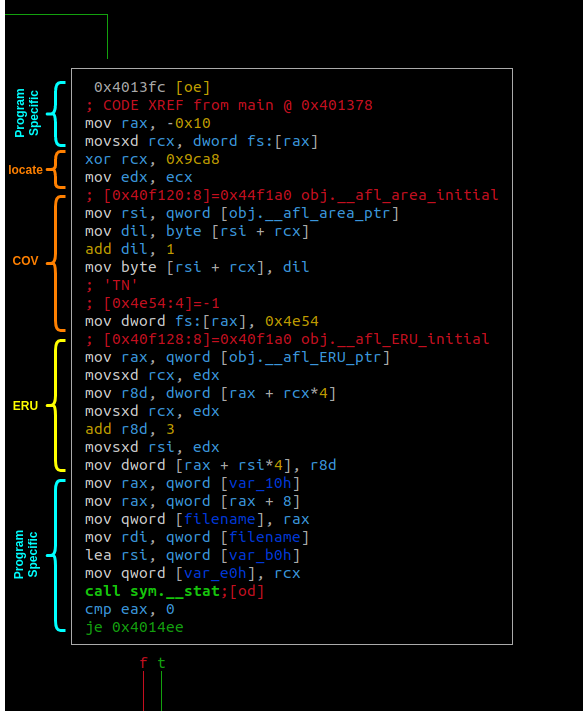
\includegraphics[width=\textwidth]{Chapter3/fuzzgoat-inst.png}
   \centering
   \caption{Instrumentation illustrated in basic blocks. This basic block contains the coverage-based and ERU-based instructions}
   \label{fig:fuzzgoat-inst}
\end{figure}

This command results in \texttt{./fuzzgoat-wfl} binary file. We pass this file to \textit{radare2} to confirm the instrumentation. Figure \ref{fig:fuzzgoat-inst} illustrates one of the basic blocks collected from the program, and different sections of the seleced basic block are specified as well. The orange sections, locate and COV, are inherited from AFL's implementation, and Waffle leverages on these parts to find the next edge index, and update the trace\_bits of the program. Next, the instructions for measuring the program's ERU come after. As stated on the figure, the first three instructions try to load the content of the edge-index of the ERU array. The loaded value is then increased by the precalculated value of the estimated resource usage of the current basic block. Then, the result of the addition is passed back into the array and updates the content of assigned pointer.

% -T: Explain the new status screen

\subsection{Fuzzing}

The steps for running Waffle are similiar to AFL; \texttt{./waffle-fuzz} gets the input and output directories, in addition to the instrumentated program:

\begin{lstlisting}[language=bash,style=CommandStyle,label={lst:wafl-fuzzgoat-fuzz}]
   cd fuzzgoat/
   waffle-fuzz -i in_dir -o out_dir -- ./fuzzgoat @@
\end{lstlisting}

Compared to AFL's status screen, Waffle informs about the state of the ERU's through fuzzing. As an example, Figure \ref{fig:status-wfl} shows a fuzzing procedure after 28 minutes of testing fuzzgoat. In \texttt{stage progress} section, \texttt{method} explains the causal method which added the selected entry (\texttt{current\_entry} under testing) to the queue; either it is discovered as a \texttt{Coverage} finding, or it is caused by a resource \texttt{Exhaustion}. Next to this section, the section \texttt{findings in depth} contains two new fields, \texttt{ERU queued} and \texttt{ERU (CAP/MAX)}. \texttt{ERU queued} specifies the queue entries which were added with an \textbf{exhaustion} feature. The other field, \texttt{ERU (CAP/MAX)} shows the average of the highest 100 ERU's which were acquired through fuzz testing, and the \texttt{MAX} value indicates the highest value for all found ERUs. 

\begin{figure}[t]
   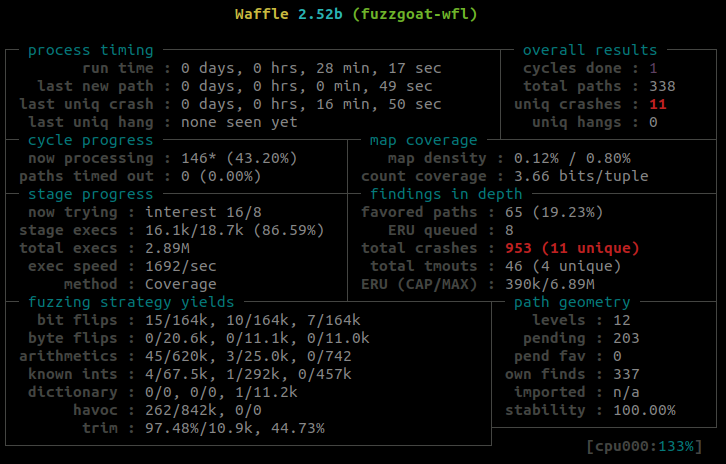
\includegraphics[width=\textwidth]{Chapter3/statusScreen-wfl.png}
   \centering
   \caption{Waffle's status screen.}
   \label{fig:status-wfl}
\end{figure}

\newpage \ \newpage